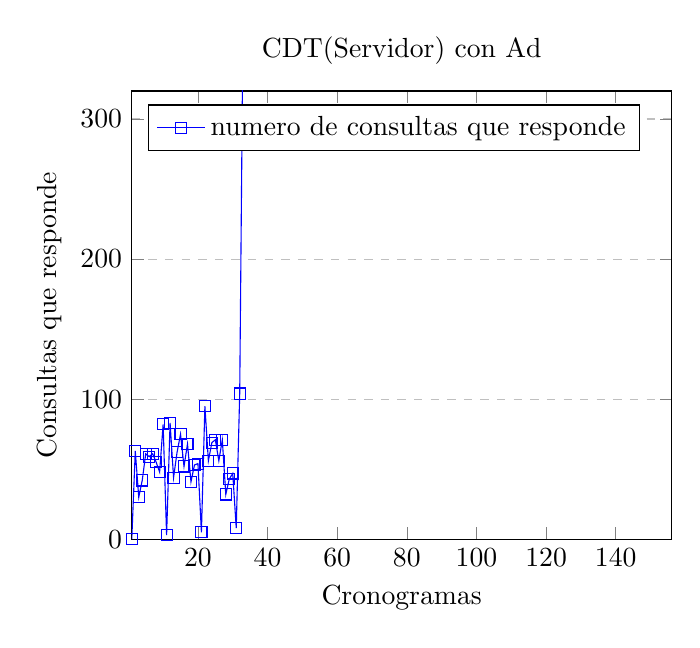
\begin{tikzpicture}
\begin{axis}[
    %CDT = carga de trabajo
    %AEPxT = Algoritmo DETRMINISTA
    title={CDT(Servidor) con Ad},
    xlabel={Cronogramas},
    ylabel={Consultas que responde},
    xmin=1, xmax=156,
    ymin=0, ymax=320,
    xtick={},
    ytick={},
    legend pos=north west,
    ymajorgrids=true,
    grid style=dashed,
]

\addplot[
    color=blue,
    mark=square,
    ]
    coordinates {
   %CARGA DE TRABAJO Servidor
(1,0)
(2,63)
(3,30)
(4,42)
(5,61)
(6,59)
(7,61)
(8,55)
(9,48)
(10,82)
(11,3)
(12,83)
(13,44)
(14,62)
(15,75)
(16,52)
(17,68)
(18,41)
(19,53)
(20,54)
(21,5)
(22,95)
(23,56)
(24,69)
(25,71)
(26,56)
(27,71)
(28,32)
(29,43)
(30,47)
(31,8)
(32,104)
(33,385)
    };
    \legend{numero de consultas que responde}

\end{axis}
\end{tikzpicture}
